\section{Aufbau}
		
	\begin{figure}
		\centering
		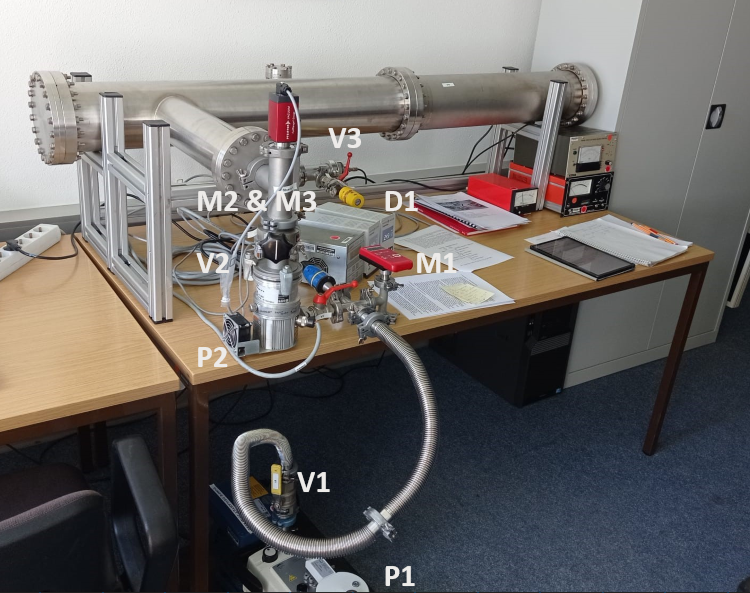
\includegraphics[width=0.8\textwidth]{"latex/images/Aufbau_beschriftet.png"}
		\caption{Ein Bild des verwendeten Versuchsaufbaus.}
		\label{fig:auf}
	\end{figure}		
	\noindent
	Beide in diesem Versuch verwndete Vakuumpumpen sind hier zu sehen.
	Bei (P1) ist am unteren Ende des Bildes die Drehschiebervakuumpumpe zu sehen, die Turbomolekularpumpe ist direkt darüber auf dem Tisch bei (P2).
	Die Drehschieberpumpe kann mittels des Ventil (V1) und die Turbopumpe mittels des Ventil (V2) abgeschoben werden.
	Zwei weitere Ventile zum Einstellen des Gleichgewichtsdruck sind das Ventil (V3) und das Dosierventil (D1) unter dem Vakuumkörper.
	Das erste relevante Messgerät ist bei (M1), welches ein kombiniertes Piezo und Pirani Vakuummeter ist.
	Bei (M2 \& M3) sind die Anzeigegeräte zu den Kaltkathoden-Vakuummetern, welche über der Turbopumpe (P2) und hinter dem Dosierventil (D1) angebracht sind.

\section{Durchführung}
	Zunächst wird die Funktionsfähigkeit der Analge überprüft und vorbereitet. 
	Dazu wird getestet ob die Drehschieberpumpe (P1) innerhalb von maximal 10 Minuten in der Lage ist einen Enddruck $P_\text{E}$ von 0,03 mbar bis 0,05 mbar zu erzeugen. 
	Ist dem nicht so, muss die Anlage auf undichte Stellen überprüft werden.
	Weiterhin wird dann mit dem bereits vorhandenen Vorvakuum, die Turbopumpe (P2) eingeschalten. 
	Um Wasseranlagen zu entfernen und Desorption vorzubeugen wird die Anlage auch einmal mit einem Heißluftfön erhitzt.
	Die Turbopumpe sollte dann in der Lage sein, einen Druck von $\SI{8 e-5}{\milli\bar}$ bis $\SI{2 e-5}{\milli\bar}$ zu erzeugen.
	Weiterhin ist es sehr wichtig, für die Auswertung einmal den Enddruck der Dreschieber- und Vakuumpumpe zu messen und zu dokumentieren.	


	\subsection{Messungen Zur Drehschieberpumpe}

		Sobald bestätigt wurde, dass der Pumpstand ausreichend dicht ist, können Evakueirungskurven aufgenommen und Leckratenmessungen durchgeführt werden.

		\subsubsection{Evakuierungskurve}

			Zunächste wird die Anlage wieder auf den Arbeitsbereich der Drehschieberpumpe belüftet, dazu muss die Turbompumpe abgeschalten werden, um Schäden an der Pumpe zu verhinden.
			Dann wird die Drehschieberpumpe abgeschoben (V1) und der Rezipient belüftet indem für ca. 5 Sekunden das Dosierventil (D1) und Ventil (V3) geöffnet wird, bis wieder Normaldruck in dem Rezipienten herscht. 
			Sobald der Rezipient wieder dicht ist, wird der Zugang zu der Drehschieberpumpe geöffnet (V1) und der Druckabfall als Funktion der Zeit vermessen. 
			Dazu werden für eine gesamt Messzeit von $\SI{600}{\second}$ alle $\SI{10}{\second}$ der Druck an dem Digitalen Vakuummeter (M1) abgelesen.
			Bei dieser Messung sollte eine Enddruck von $P_\text{E}$ zwischen 0,1 mbar und 0,08 mbar erreicht werden.
			Diese Messung wird dann 3-mal wiederholt.

		\subsubsection{Leckratenmessung}

		 	Die Leckratenmessung wird durchgeführt indem mittels des Nadelventils (D1) ein Gleichgewichtsdruck $p_\text{g}$ eingestellt und dann bei weithin offenem Dosierventil die Pumpe vom System abgeschoben wird (V1).
			Den darauf folgenen Druckanstieg wird dann als Funktion der Zeit über $\SI{200}{\second}$ in $\SI{10}{\second}$ Abständen gemessen. 
			Diese Messung wird mit 4 Gleichgeichtsdrücken $p_\text{g} = 0,4; 10; 40; \SI{80}{\milli\bar}$ und jeweils 3 Messreihen durchgeführt.

	\subsection{Messung zur Turbopumpe}

		Die Messungen zu der Turbopumpe (P2) laufen analog zu denen der Drehschieberpumpe. 
		Es ist hier wichtig darauf zu Achten, dass bevor die Turbopumpe eingeschalten wird, bereits eine Vorvakuum von mindestens $\SI{10e-1}{\milli\bar}$ mit der Drehschieberpumpe erzeugt wurde.
		
		\subsection{Evakuierungskurve}

			Dieses mal wird der Rezipient nicht komplett belüftet damit die Turbopumpe direkt starten kann. 
			Als Startdruck  wird mit dem Dosierventil bei laufender Pumpe ein Druck von $\SI{1.6e-3}{\milli\bar}$ eingestellt.
			Dann wird das Ventil (V3) geschlossen und das zunehmende Vakuum in einer $p(t)$-Kurve über $\SI{200}{\second}$ alle $\SI{10}{\second}$ aufgenommen.
			Auch diese Messung wird 3 mal wiederholt.

		\subsection{Leckratenmessung}

			Die Leckratenmessungen der Turbopumpe läuft auch sehr analog zu denen der Drehschieberpumpe, es werden jediglich nur über $\SI{120}{\second}$ Werte aufgenommen. 
			Und die Gleichgewichtsdrücke von denen die Leckratenmessung startet sind: $(1 \& 2)\cdot10^{-4}$ mbar und $(5 \& 7)\cdot10^{-5}$ mbar.
			Zum Abschiebern der Turbopumpe wird nun aber das Ventil (V2) verwendet.
